\section{数据预处理与分析}

为构建有效的种植策略优化模型,首先需要对研究背景中涉及的基础数据进行系统性的分析与处理。本章将围绕耕地资源特性、农作物种植条件及经济效益指标三个核心维度展开,旨在明确模型构建所需的基本参数与约束条件。

\subsection{耕地资源分析}

该乡村的耕地资源主要由露天耕地与大棚构成。根据附件数据,我们汇总了各类土地的面积与分布情况。图\ref{fig:land_distribution}直观地展示了不同类型土地资源的面积占比。

\begin{figure}[htbp]
    \centering
    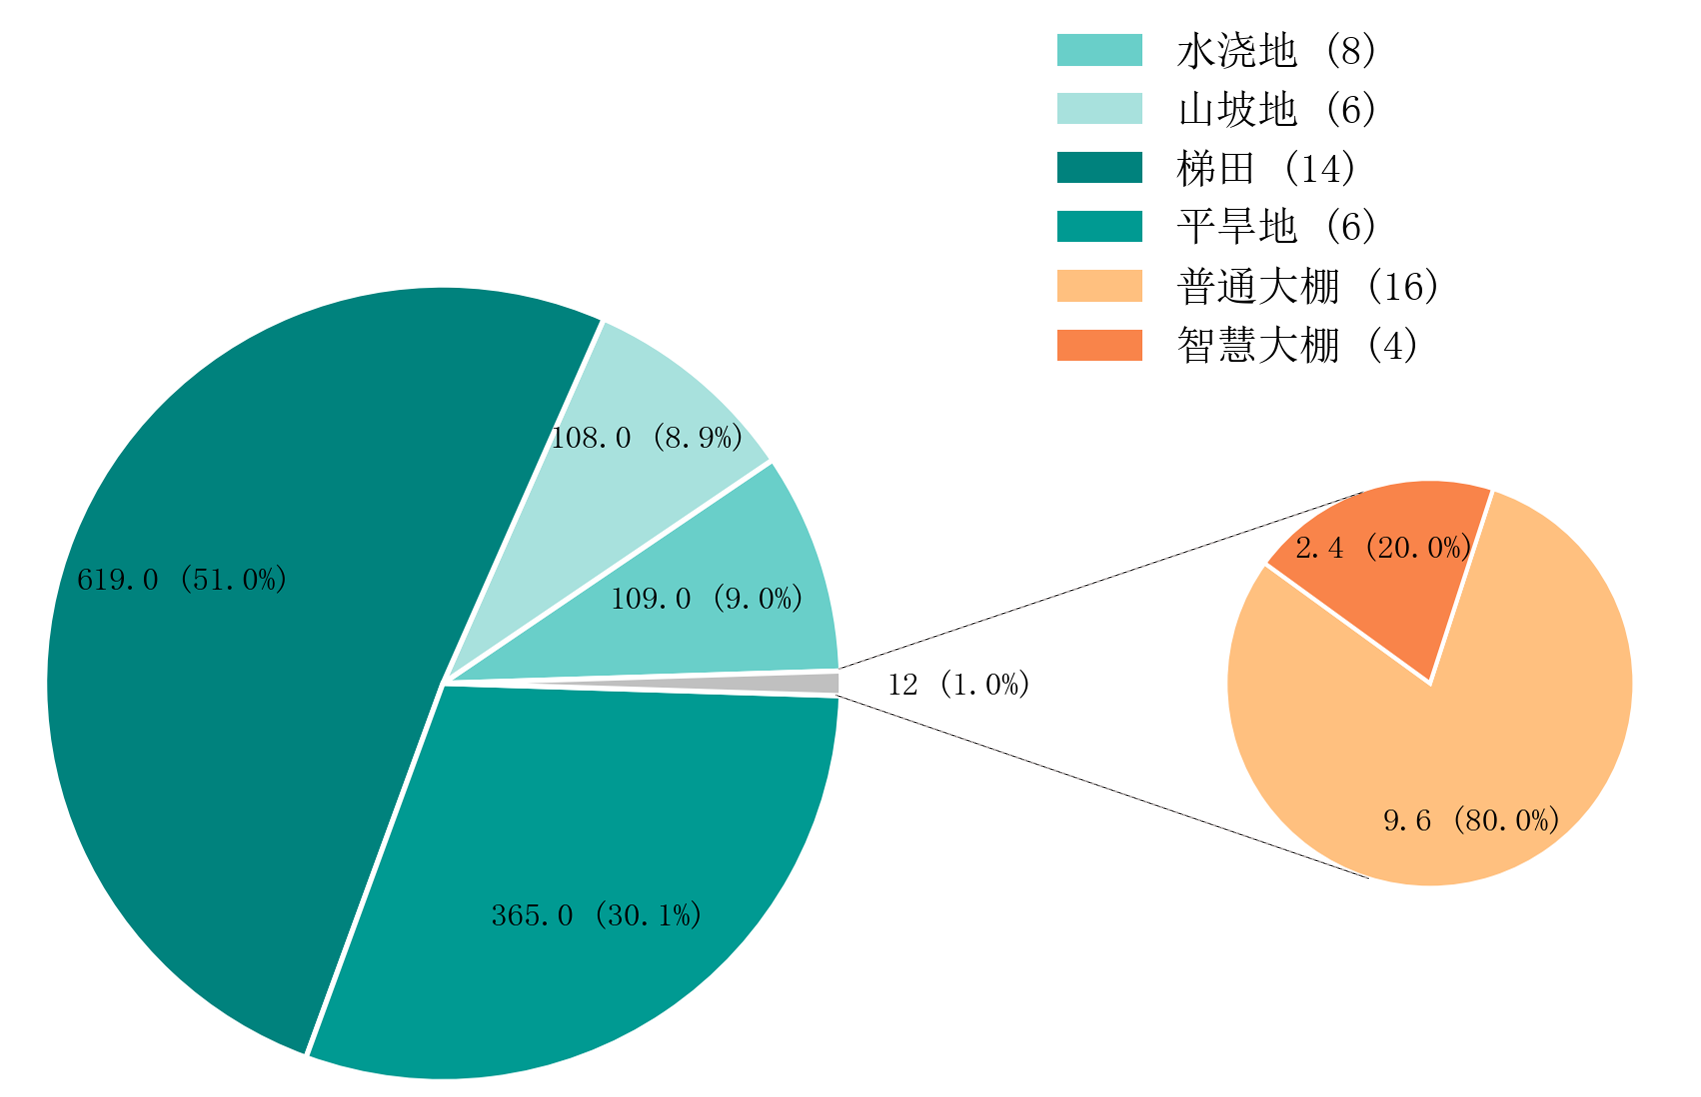
\includegraphics[width=0.8\textwidth]{figs/2数据分析与预处理/土地类型分布.png}
    \caption{土地类型分布情况}
    \label{fig:land_distribution}
\end{figure}

根据资料,不同类型的土地其物理特性与配套设施存在差异,从而决定了其适宜种植的作物类型与种植模式。
\begin{itemize}
    \item \textbf{平旱地(A)、梯田(B)与山坡地(C)}:这三类土地缺乏灌溉条件,农业生产完全依赖自然降水。此类土地环境适合种植耐旱、需水较少的单季粮食作物,不适宜水稻的生长。
    \item \textbf{水浇地(D)}:该类土地具备完善的灌溉设施,能够保障作物生长所需的水分。由于水稻的生长周期较长,若种植水稻则为单季种植。此外,该地块也可用于两季蔬菜的种植。从水资源供给角度看,第一季水源充足,适宜种植需水量较高的蔬菜;第二季为满足耐寒和简化管理的需求,种植作物限定为大白菜、白萝卜或红萝卜中的一类。
    \item \textbf{普通大棚(E)}:作为一种利用塑料薄膜或玻璃覆盖形成的设施农业,大棚内部形成了可控的小气候环境。其维护成本较高,因此不适宜种植附加值较低的粮食作物。棚内空间相对密闭,高温高湿的环境使得部分作物易受病虫害影响。同时,其土层较浅,不适合根系发达的蔬菜作物。因此,普通大棚适宜进行两季作物轮作,第一季可种植多种蔬菜,而第二季则种植对湿度和温度要求较低的食用菌。
    \item \textbf{智慧大棚(F)}:作为普通大棚的升级版本,智慧大棚通过现代技术手段实现对棚内温度、湿度、光照等环境因子的实时监控与调控。优化的生长环境使其能够支持两季蔬菜的种植,从而提高土地利用效率与产出。
\end{itemize}

\subsection{农作物种植条件分析}

基于对土地特性的分析,我们进一步梳理了各类农作物的具体种植要求。不同作物在作物类别、适种耕地、耕种时序等方面存在明确的划分,这些构成了种植决策的基本约束。表\ref{tab:crop_requirements}系统地总结了所有可选作物的种植要求。

\begin{table}[htbp]
    \centering
    % 使用 threeparttable 环境来管理标题、表格主体和脚注
    \begin{threeparttable}
        \caption{优化后的农作物种植要求}
        \label{tab:crop_requirements_optimized_1}
        % 使用 tabularx 环境,并设置总宽度为列宽 \columnwidth
        % X 列是一种特殊的列,可以自动伸展以填充可用空间
        \begin{tabularx}{\columnwidth}{l l >{\raggedright\arraybackslash}X l}
            \toprule
            作物类别 & 作物子类/名称 & 种植耕地 & 耕种时期 \\
            \midrule
            % 使用 \multirow 合并“粮食”类别下的三行
            \multirow{3}{*}{粮食}
            & 豆类 (黄豆、黑豆、豌豆等) & A, B, C & 单季种植 \\
            \addlinespace % 在行之间增加一点垂直空间,使分组更清晰
            & 谷物及薯类 (小麦、玉米、南瓜、红薯等) & A, B, C & 单季种植 \\
            \addlinespace
            & 水稻 & D & 单季种植 \\
            \midrule
            % 使用 \multirow 合并“蔬菜”类别下的三行
            \multirow{3}{*}{蔬菜}
            & 豆类 (豇豆、刀豆、芸豆) & D, E, F & 第一、二季 \\
            \addlinespace
            & 常见蔬菜 (番茄、黄瓜、菠菜等) & D, E, F & 第一、二季 \\
            \addlinespace
            & 大白菜、萝卜 & D & 第二季 \\
            \midrule
            食用菌 & 榆黄菇、香菇、羊肚菌等 & E & 第二季 \\
            \bottomrule
        \end{tabularx}
        % 使用 tablenotes 环境添加表格的脚注
        \begin{tablenotes}[flushleft]
            \footnotesize % 设置脚注字体为小号
            \item[备注] A=平旱地, B=梯田, C=山坡地, D=水浇地, E=普通大棚, F=智慧大棚。
        \end{tablenotes}
    \end{threeparttable}
\end{table}


从表\ref{tab:crop_requirements}可知,作物的种植选择与土地类型和种植季节严格对应。例如,粮食作物主要在A、B、C类土地上单季种植,而蔬菜和食用菌则主要分布在D、E、F类土地上,并存在明确的季节划分。

\subsection{经济效益指标分析}

为了对不同种植方案的优劣进行量化评估,需要分析各农作物的经济效益。我们基于2023年的相关统计数据,对该年度的作物总产量分布和单位亩利润进行了可视化分析。

图\ref{fig:production_distribution_2023}展示了2023年各种农作物的总产量情况。从中可以看出不同作物在乡村农业生产中所占的比重。

\begin{figure}[htbp]
    \centering
    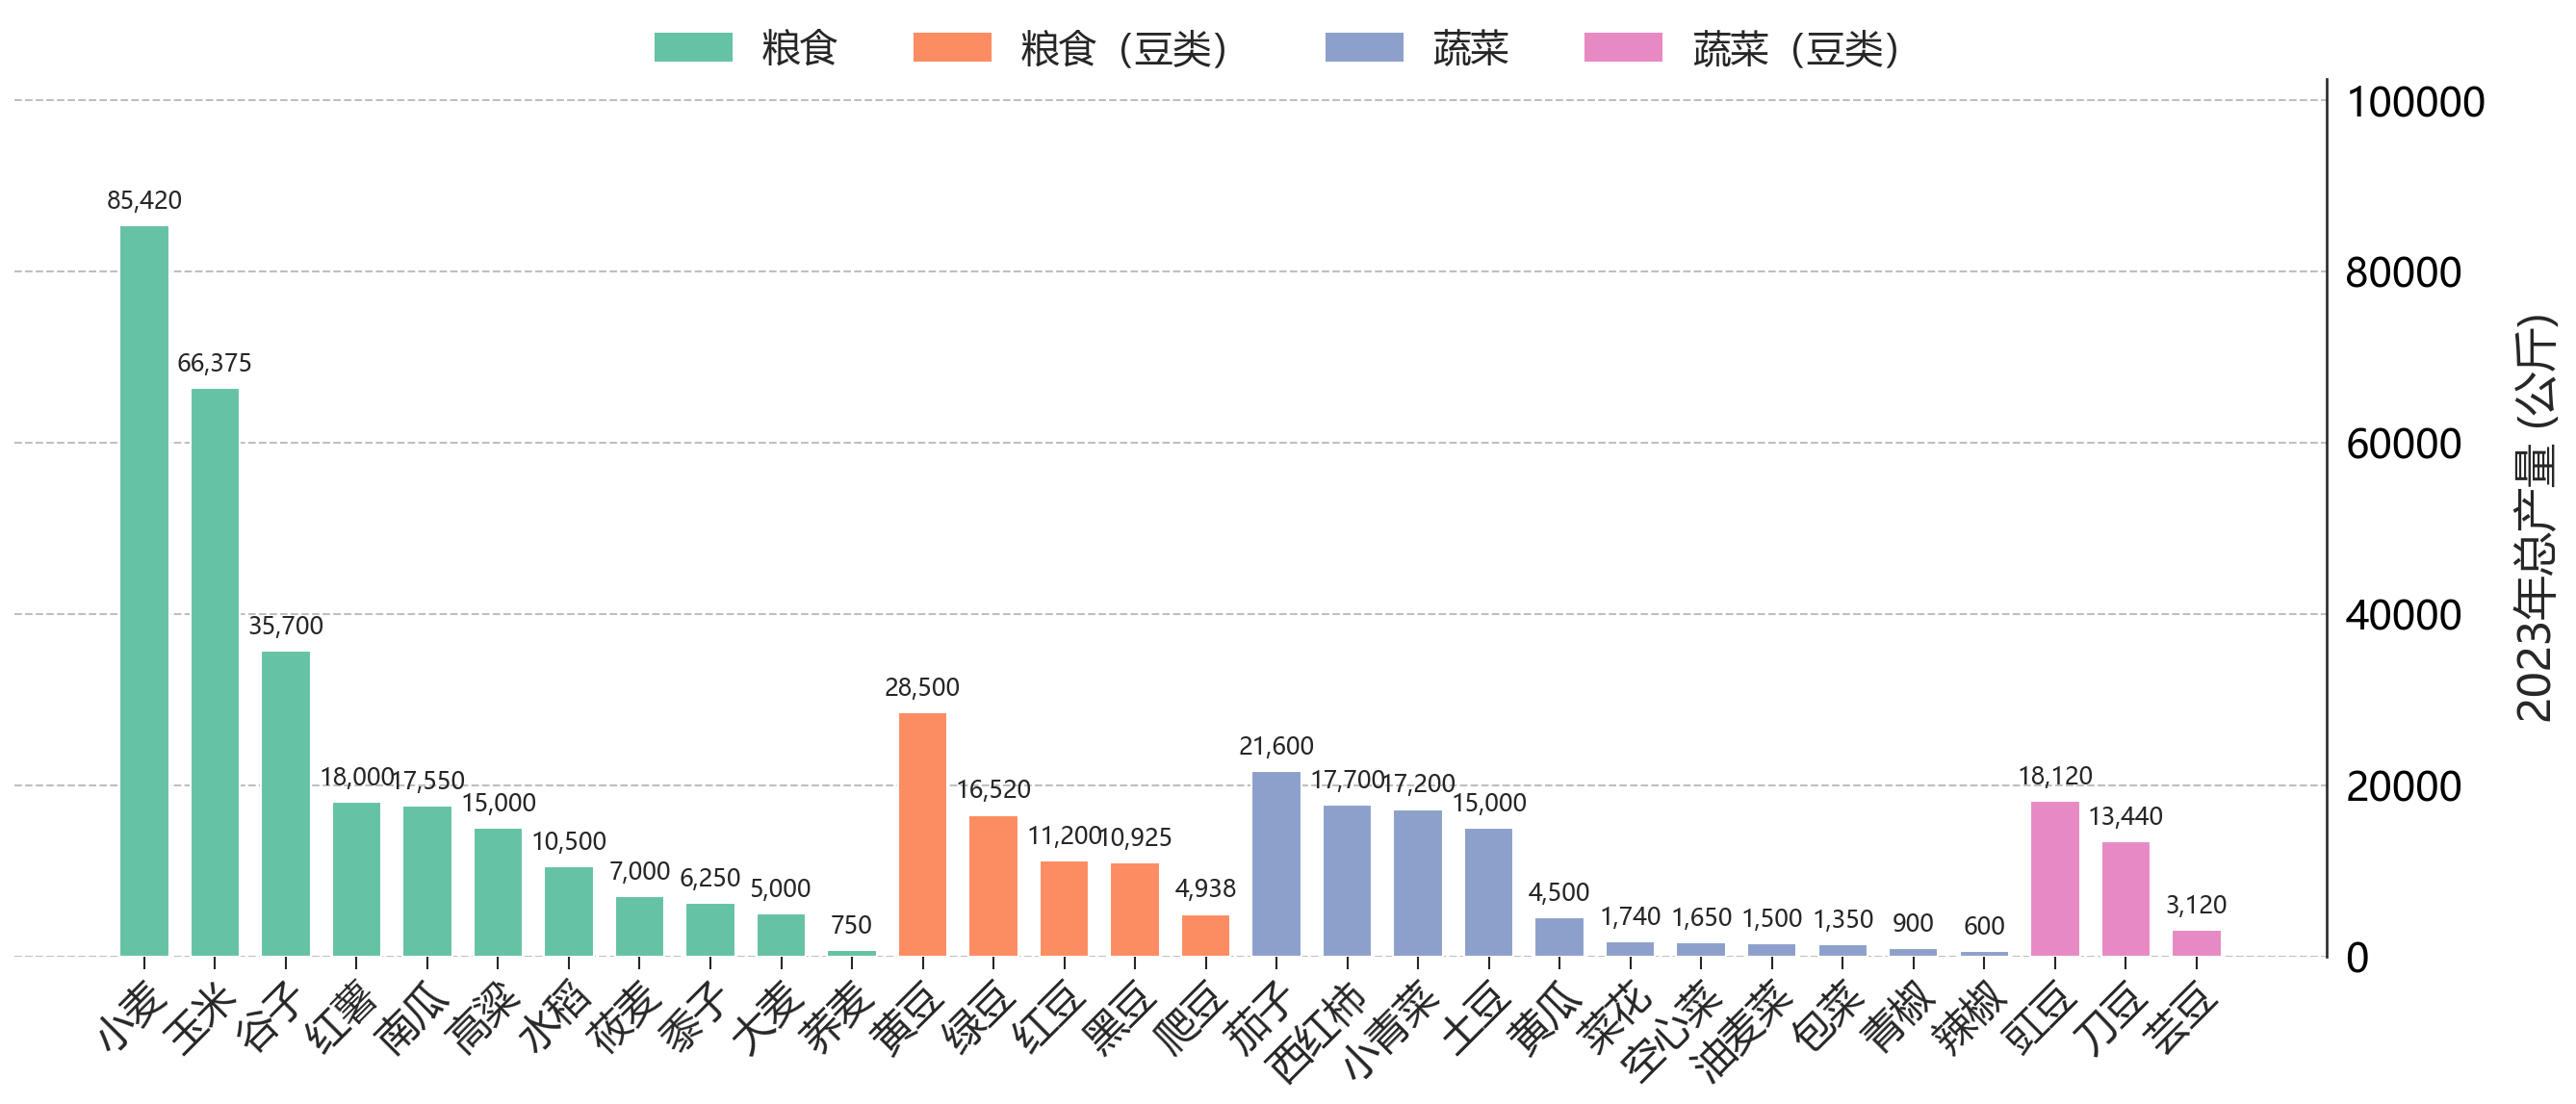
\includegraphics[width=0.8\textwidth]{figs/2数据分析与预处理/2023年产量分布.png}
    \caption{2023年农作物总产量分布}
    \label{fig:production_distribution_2023}
\end{figure}

图\ref{fig:profit_per_mu_2023}则揭示了不同作物在2023年的单位亩利润水平。单位面积的盈利能力是衡量作物经济价值的核心指标。

\begin{figure}[htbp]
    \centering
    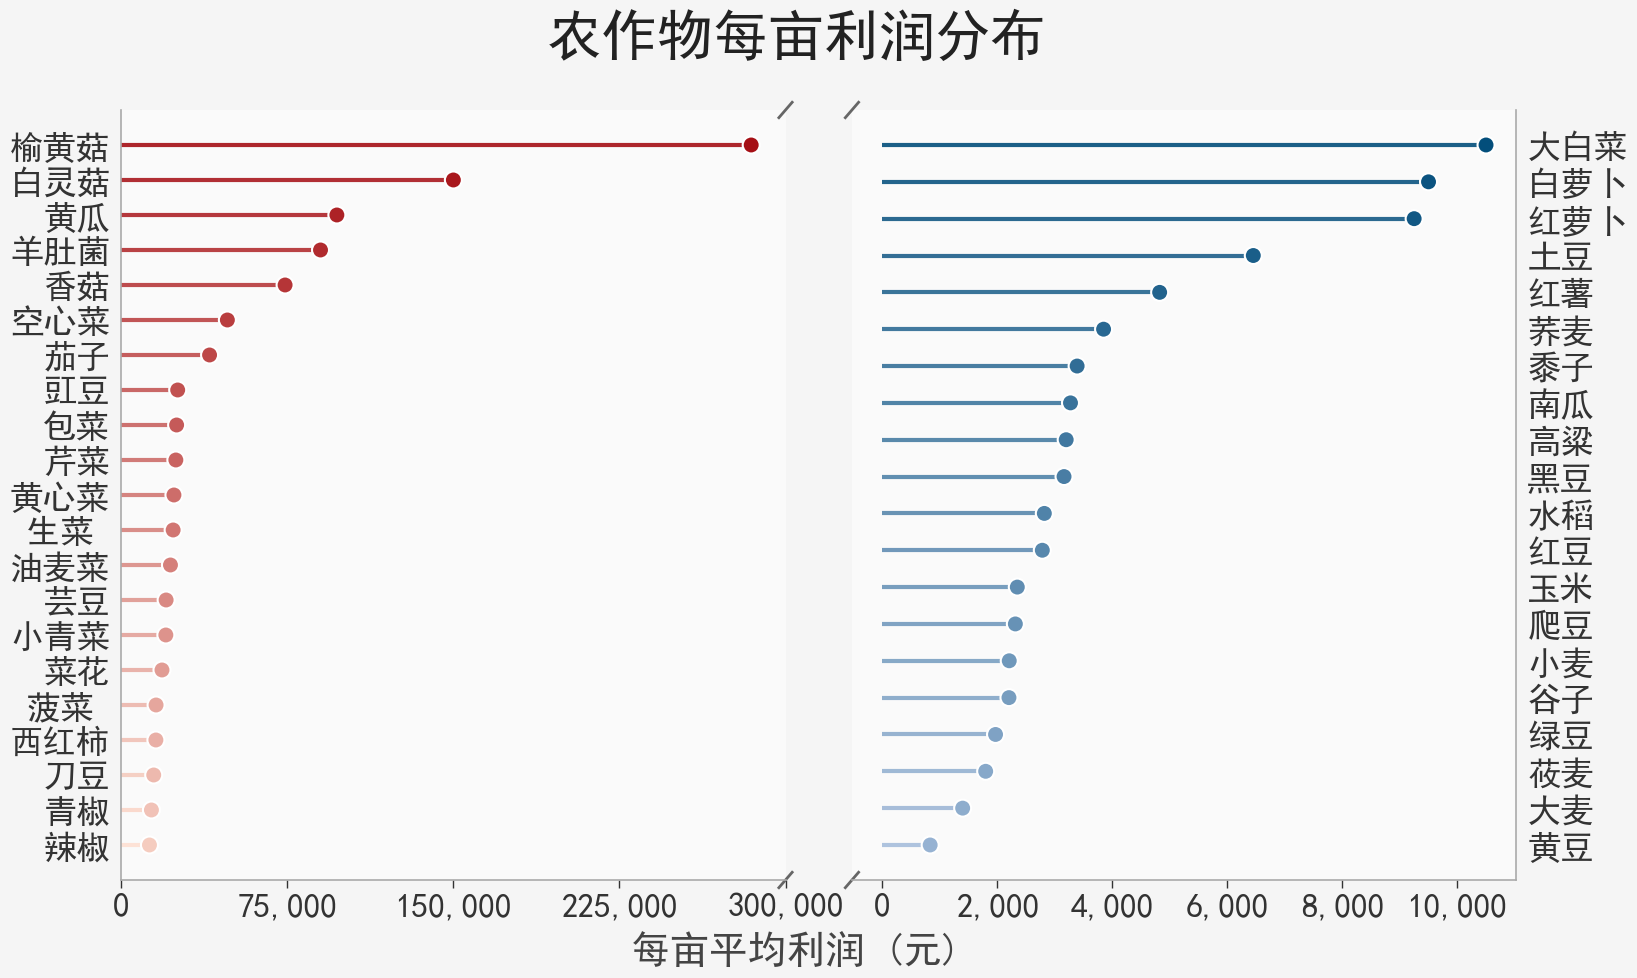
\includegraphics[width=0.8\textwidth]{figs/2数据分析与预处理/2023年单位亩利润.png}
    \caption{2023年各作物单位亩利润}
    \label{fig:profit_per_mu_2023}
\end{figure}

为统一衡量标准,我们将单位亩利润作为评估经济效益的基础。对于任意一种作物$i$,其单位亩利润$P_i$的计算方式如下:
\begin{equation}
    P_i = Y_i \times S_i - C_i
    \label{eq:profit}
\end{equation}
其中,$Y_i$表示作物$i$的单位亩产量(斤/亩),$S_i$表示其销售价格(元/斤),$C_i$表示其单位亩种植成本(元/亩)。通过此公式,我们将原始数据转化为直接用于优化模型目标函数的关键经济参数。

综上所述,通过对耕地资源、作物种植条件和经济效益指标的系统分析与处理,我们为后续构建多目标、多约束的种植策略优化模型奠定了坚实的数据基础。
